\documentclass{standalone}
\usepackage{tikz}
\usetikzlibrary{arrows.meta, positioning, calc}

\begin{document}

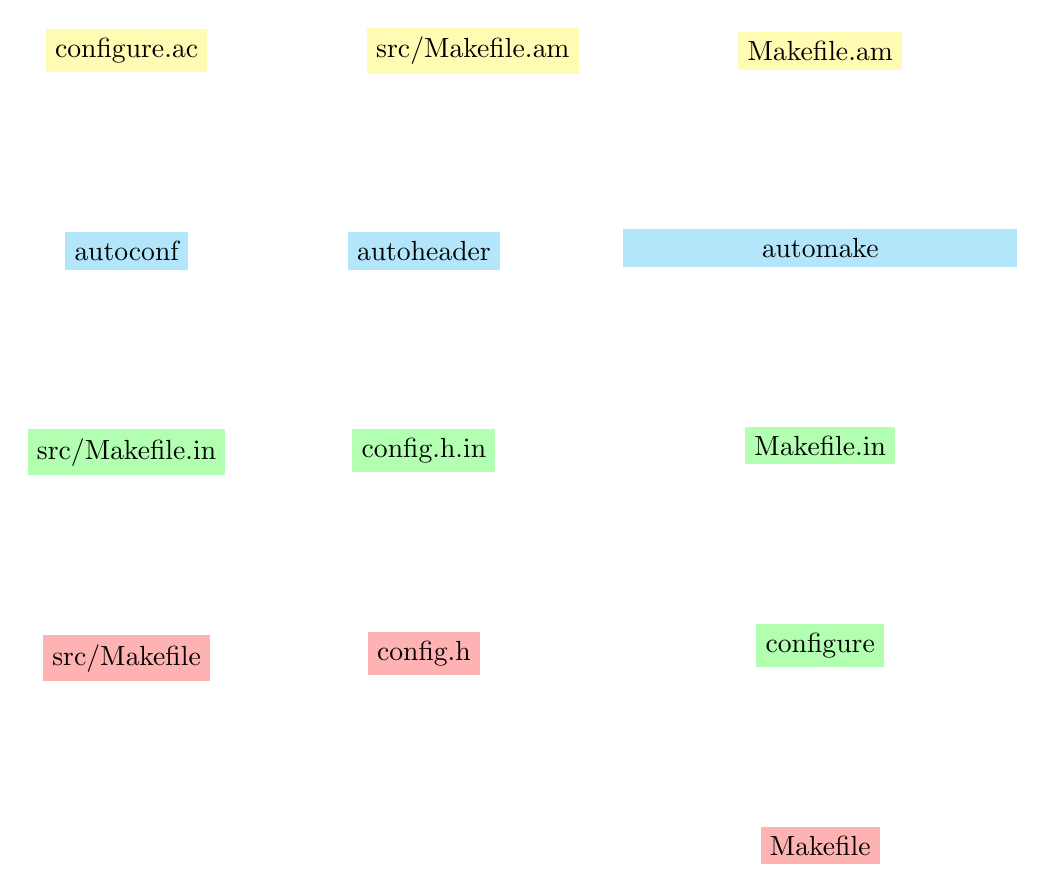
\begin{tikzpicture}[ thick, ->, >=Stealth, node distance = 2cm, ]

    \tikzstyle{ every node/.style}=[draw, rectangle, rounded corners, align=center, minimum height=10mm]
    \tikzstyle{tool}=[fill=cyan!30]
    \tikzstyle{written}=[fill=yellow!30]
    \tikzstyle{generated}=[fill=green!30]
    \tikzstyle{usergenerated}=[fill=red!30]


% Nodes
\node[written] (configure_ac) {configure.ac};
\node[written, right=of configure_ac] (src_makefile_am) {src/Makefile.am};
\node[written, right=of src_makefile_am] (makefile_am) {Makefile.am};

\node[tool, below=of configure_ac] (autoconf) {autoconf};
\node[tool, below=of makefile_am, minimum width=5cm] (automake) {automake};
\node[tool, right=of autoconf, align=center] (autoheader) {autoheader};

\node[generated, below=of autoheader] (config_in) {config.h.in};
\node[generated, below=of autoconf] (makefile_in_src) {src/Makefile.in};
\node[generated, below=of automake] (makefile_in) {Makefile.in};

\node[generated, below=of makefile_in] (configure) {configure};

\node[usergenerated, below=of config_in] (config_h) {config.h};
\node[usergenerated, below=of makefile_in_src] (makefile_src) {src/Makefile};
\node[usergenerated, below=of configure] (makefile) {Makefile};

% Arrows
% \draw[->] (autoheader) -- (config_in);
% \draw[->] (configure_ac) -- (autoconf);
% \draw[->] (autoconf) -- (makefile_in_src);
% \draw[->] (autoconf) -- (configure);
% \draw[->] (automake) -- (makefile_in);
% \draw[->] (config_in) -- (config_h);
% \draw[->] (configure) -- (config_h);
% \draw[->] (makefile_in_src) -- (makefile_src);
% \draw[->] (configure) -- (makefile_src);
% \draw[->] (makefile_in) -- (makefile);
% \draw[->] (configure) -- (makefile);

% % Legend
% \node[draw=none, fill=none, below=of makefile, align=left] (legend) {
%     \begin{tabular}{ll}
%         \node[written]{}; & Written by the developer \\
%         \node[tool]{}; & Tools used by the developer generally through autoreconf \\
%         \node[generated]{}; & Generated by the developers, as a result of autoreconf \\
%         \node[usergenerated]{}; & Generated by the person building the software \\
%     \end{tabular}
% };

\end{tikzpicture}

\end{document}
